\section{System Model}
\label{sec:problem}

\subsection{Assumptions}
We assume that parking spaces in question are located in a parking lot with a known layout which consists of multiple adjacently placed parking spots and vehicles are expected to be parked in a vertical manner. While the proposed system can be used in both indoor and outdoor parking lots, parallel parking is not supported since it introduces additional challenges in distinguishing between parked vehicles and other objects as well as changing the parking lot layout. However, the proposed system can be extended to support parallel parking in the future, possibly by training the model with additional data from parallel parking scenarios.

\subsection{Problem Statement}
In the proposed scenario, the objective is to detect the presence of a vehicle in a parking space using wireless signals. The system is designed to operate in a parking lot with multiple adjacent parking spaces, where each space can either be occupied by a vehicle or remain empty. The goal is to accurately identify the occupancy status of each parking space based on the received wireless signals, without requiring dedicated sensors for each spot. 

\subsection{System Overview}

\begin{figure}[H]
\begin{center}
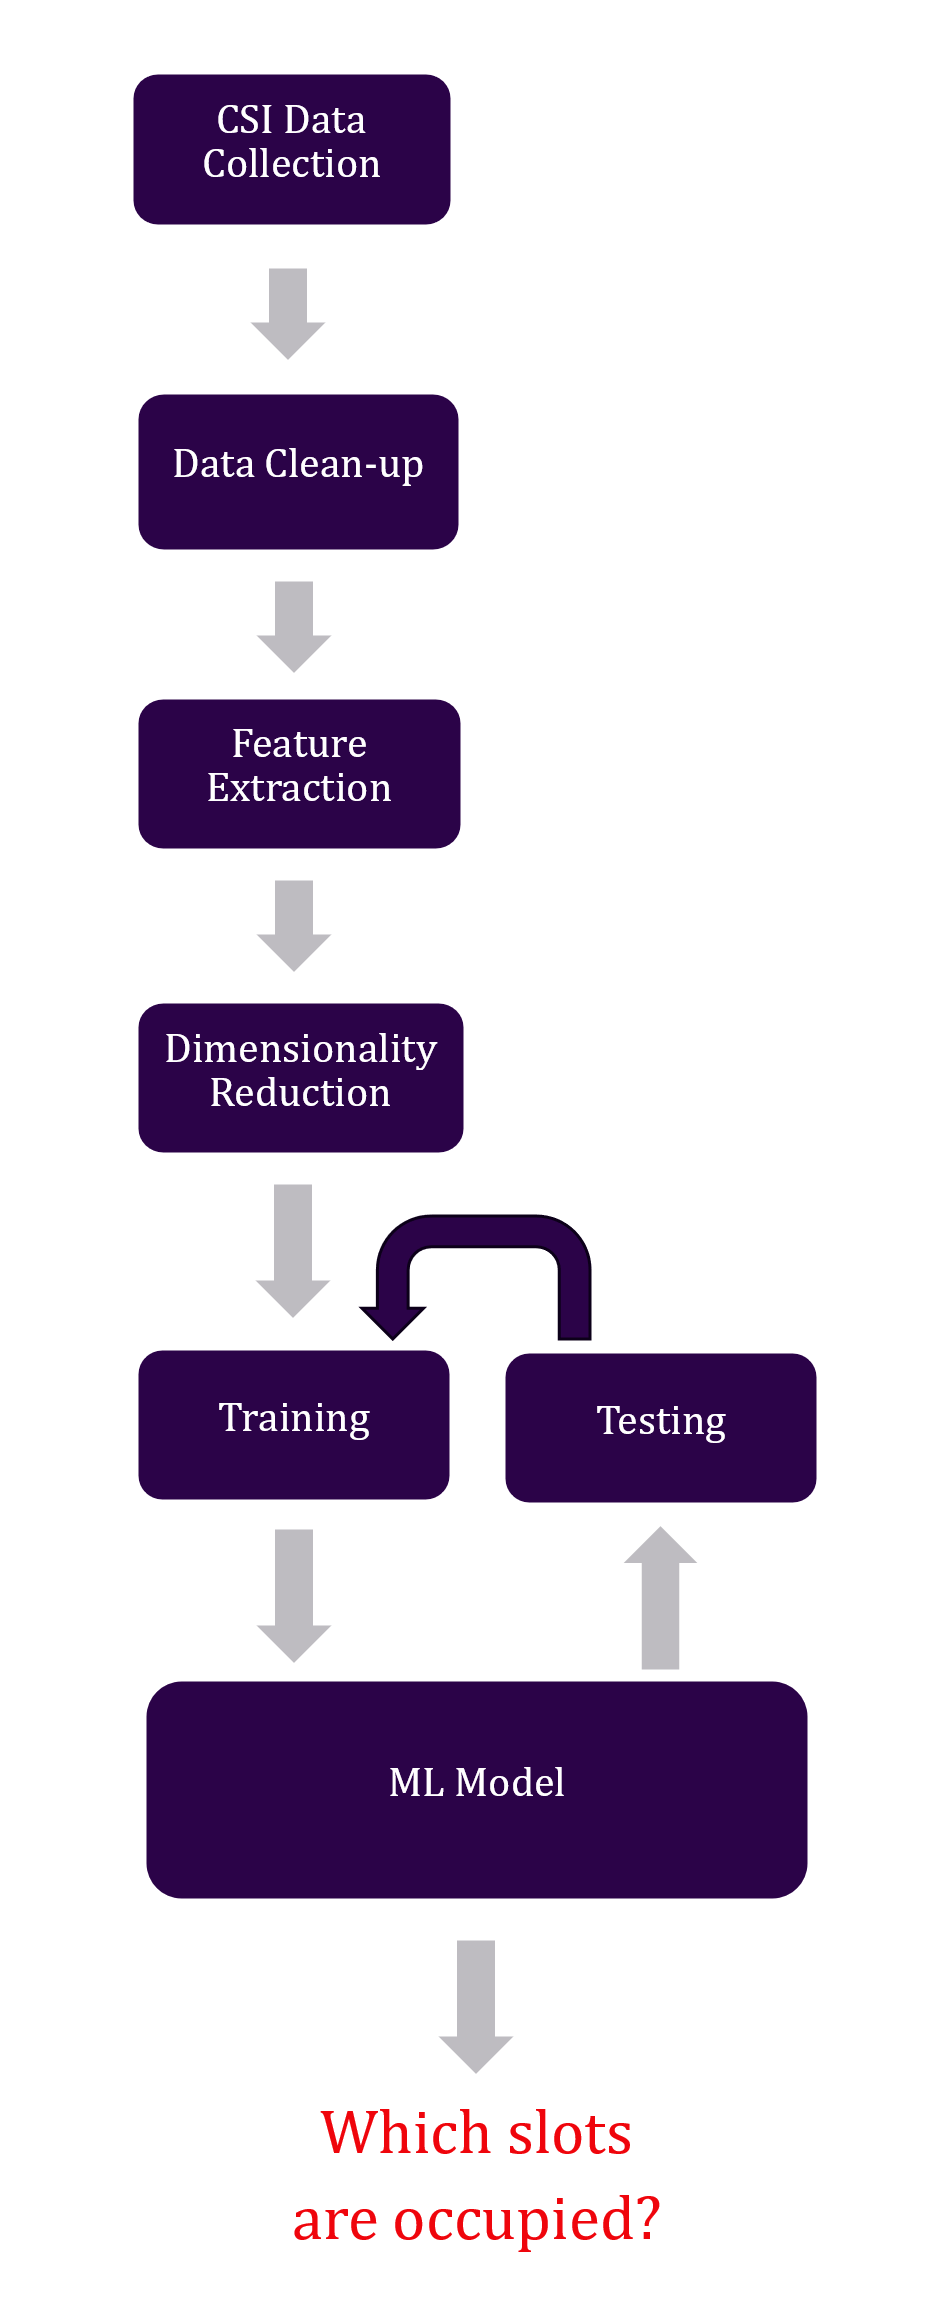
\includegraphics[width=8cm]{Figures/system_design.png}\vspace{0mm}
\caption{The architecture of the proposed system}\vspace{0mm}
\label{fig:system_design}
\end{center}
\end{figure}

The proposed system follows a multi-stage process as illustrated in Figure~\ref{fig:system_design}. Each stage plays a crucial role in transforming raw wireless signals into accurate parking occupancy information.

\subsubsection{CSI Data Collection}
The first step involves collecting Channel State Information (CSI) in various parking scenarios. This data captures the multipath propagation characteristics of Wi-Fi signals, which are affected by the presence and absence of vehicles. 

\begin{figure}[H]
    \begin{center}
        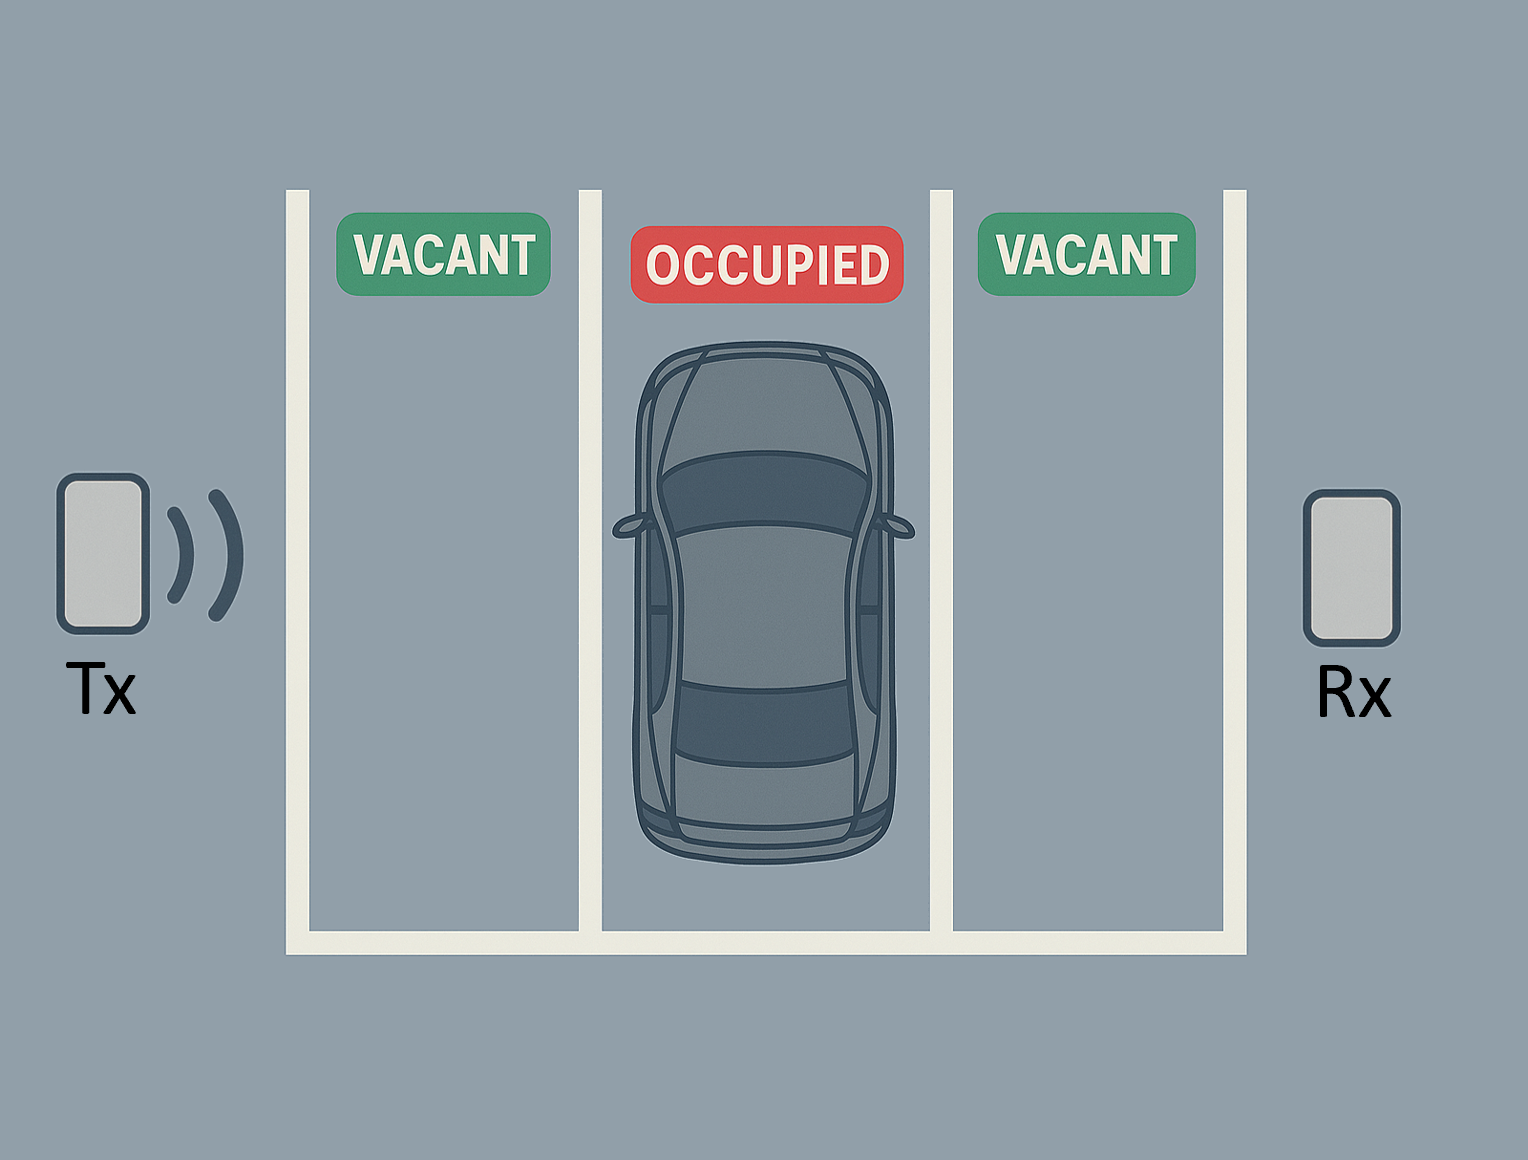
\includegraphics[width=8cm]{Figures/layout.png}\vspace{0mm}
        \caption{Data collection setup}\vspace{0mm}
        \label{fig:data_collection_setup}
    \end{center}
\end{figure}

    The data collection setup is shown in Figure~\ref{fig:data_collection_setup}. The system consists of a transmitter (Tx) and a receiver (Rx), where the transmitter sends Wi-Fi signals to the receiver. The receiver captures the CSI data, which includes information about the amplitude and phase of the received signals. This data is collected over time to create a comprehensive dataset that reflects different parking scenarios, including different combinations of occupancy states across multiple parking spaces between the transmitter and receiver. 

\subsubsection{Data Cleaning}
The raw CSI data collected often contains noise and outliers due to environmental factors and hardware imperfections. Therefore, a data cleaning phase is essential. This involves removing any irrelevant or corrupted data points, filtering out noise, and normalizing the data to ensure consistency. Techniques such as median filtering, moving average smoothing, and outlier detection algorithms can be employed to enhance the quality of the CSI data.

\subsubsection{Feature Extraction}
Next, relevant features are extracted from the cleaned CSI data. CSI provides information about the channel frequency response (CFR) across multiple orthogonal frequency-division multiplexing (OFDM) subcarriers. For each packet received at time $t$, the CSI for the $k$-th subcarrier, $H(f_k, t)$, can be represented as a complex number:
\[
H(f_k, t) = |H(f_k, t)| e^{j \angle H(f_k, t)} = a + jb
\]
where $H^*(f_k, t)$ is the complex conjugate of $H(f_k, t)$, $a$ and $b$ are the real and imaginary parts of the CSI, respectively. The amplitude and phase of the CSI can be expressed as:
\begin{equation}
    \text{Amplitude}(f_k, t) = |H(f_k, t)| = \sqrt{a^2 + b^2}
\end{equation}
\begin{equation}
    \text{Phase}(f_k, t) = \angle H(f_k, t) = \tan^{-1}\left(\frac{b}{a}\right)
\end{equation}

This extraction process provides a an amplitude and phase value for each subcarrier at each time instance.

\subsubsection{Dimensionality Reduction}
To reduce the dimensionality of the extracted features and improve computational efficiency, dimensionality reduction techniques such as Principal Component Analysis (PCA) or t-Distributed Stochastic Neighbor Embedding (t-SNE) can be employed. These techniques help to retain the most significant features while discarding redundant or irrelevant information. The reduced feature set is then used for training the machine learning model.

\subsubsection{Model Training and Testing}
Subsequently, a machine learning model is trained using the extracted features and corresponding ground truth labels which consists of the occupancy state of the parking spaces. For example, if the parking lot has 10 parking spaces, the occupancy state can be represented as a binary vector of length 10, where each element indicates whether the corresponding parking space is occupied (1) or empty (0). While the proposed system can be trained with any machine learning model, neural networks are particularly effective due to their ability to capture complex patterns in the data as well as their suitability for time-series data based on signal processing. Additionally, the model is tested using a separate validation dataset to evaluate its performance and generalization capabilities.
